\chapter{Installation on Windows platform}\label{sec:WinInstall}

\paragraph{}The FA$\mu$ST project is based on an C++ library available for both UNIX and Windows environments. CMake has been choose to build the project FA$\mu$ST because it is an open-source, cross-platform family of tools designed to build, test and package software.

\paragraph{}This chapter presents the steps to install the FA$\mu$ST tools on the Windows platform. First section \ref{sec:WinGettingStarted} presents the basic installation of FA$\mu$ST and second section \ref{sec:WinCustomInstall} corresponds to the advanced  installation.


\section{Getting Started} \label{sec:WinGettingStarted}

\subsection{Required tools}\label{sec:WinRequired}
The installation of the FA$\mu$ST tools depends on other components to be installed in order to run properly. 
\begin{enumerate}

\item \textbf{Install CMake} for building the FA$\mu$ST tools. 
From \url{https://cmake.org/download/}, download Binary distributions correspond to your environment (in our case  cmake-3.6.1-win64-x64.zip). The directory of binary must be add to the environment PATH of your system if you want to use the cmake command line tool. 

% \item \textbf{Install 7-Zip} from \url{http://www.7-zip.org/}. 7-Zip is a file archiver used to extract external library files. Please verify that \texttt{7z.exe} is present in your environment PATH of your system.

\item \textbf{Install Matlab} if not already done (MATLAB R2015b in our case). The builder of the FA$\mu$ST tools automatically checks your Matlab root directory if your \texttt{matlab.exe} is present in your environment Path and/or if your Matlab installation has been performed in a default directory like \texttt{"C:/Program Files/MATLAB/<R2015b>/bin/matlab.exe"} or \texttt{"C:/Program Files (x86)/MATLAB/<R2015b>/bin/matlab.exe"}. In case of several versions of Matlab installed in your system, you can force the directory of your preferred version of Matlab using the following system variable : \\
\texttt{MATLAB\_EXE\_DIR="C:/Program Files/MATLAB/<R2015b>/bin/matlab.exe"}

\textit{Note for the case of using the compiler MinGW :} In Matlab, you must install MinGW version 4.9.2 from MATLAB using the \textbf{ADDON menu}. For more detail, please follow the instruction given in following link :  
\url{http://fr.mathworks.com/help/matlab/matlab_external/install-mingw-support-package.html}. For that, you must have a id session for Mathwork. It is easy to create. 
Current this latest step, an environment variable called MW\_MINGW64\_LOC is automatically generated. 

\item \textbf{Install C++ Compiler:} Both \textbf{Microsoft visual C++} and \textbf{MinGW "Minimalist GNU for Windows"} compiler have been tested. If you are friendly with Unix tools and command line terminal, preferd \textbf{MinGW "Minimalist GNU for Windows"} C++ compiler. Otherwise, if you are more familiar with the graphical user interface, prefer the \textbf{Microsoft visual C++} compiler. The version of the C++ compiler must be coherent with the version of your Matlab version. In this documentation, the version of our C++ compiler corresponds to Matlab 2014 and 2015. If you use an other version of Matlab, please refer to the Mathworks website \url{http://fr.mathworks.com/support/compilers/<R20XXa>}.

\paragraph{}For \textbf{Microsoft visual C++} installation :
\begin{itemize}
\item Download and install Microsoft Visual C++ 2013 professional from \url{https://www.microsoft.com/en-US/download/details.aspx?id=44916}
% \item Download and install Microsoft .NET Framework 4
% \item Download and install Microsoft SDK 7.1
\end{itemize}

\paragraph{}For \textbf{MinGW} installation :
\begin{itemize}
\item Download Mingw in \url{https://sourceforge.net/projects/mingw/files/latest/download?source=files}
\item Launch install file and choose MINGW version 4.9.2 for mexFunction compatibility 
\item The directory of binary must be add to the environment PATH. 

\item \textit{Note for make tool :} In a terminal command, type \texttt{make}. if it doesn't exist, please check if \textbf{make.exe} file is present in MINGW install directory. if not, you can copy and rename mingw32-make.exe to make.exe
\end{itemize}

\end{enumerate}


\subsection{Required packages}\label{sec:WinRequiredPackages}
\paragraph{}Here is a list of packages used in the FA$\mu$ST project.
\begin{itemize}
\item \textbf{Eigen} is a C++ template library for linear algebra: matrices, vectors, numerical solvers, and related algorithms (see \url{http://eigen.tuxfamily.org}). This library is automatically install: there are nothing to do (see the directory "./externals").
\item \textbf{OpenBLAS} is an optimized BLAS library based on GotoBLAS2 1.13 BSD version. (see \url{http://www.openblas.net}). To install OpenBlas, refer to \url{https://github.com/xianyi/OpenBLAS/wiki/Installation-Guide}. 

\end{itemize}


\subsection{Basic build and Installation}\label{sec:WinBasicInstall}
\paragraph{}When prerequisites listed in previous section \ref{sec:WinRequired} are checked, the FA$\mu$ST installation can be done. 
First download the FA$\mu$ST package on the website  \url{http://faust.gforge.inria.fr/}. 

Depending to your C++ compiler (MinGW or Visual studio), refer to the right part and follow the given instructions.
\\

\subsubsection{Using MinGW compiler:}
\label{sec:WinMinGWBasicInstall}

\begin{itemize}
\item Open a command terminal
\item Place you in your local FA$\mu$ST directory (NOTE: don't use any special character in your FAUST directory path, for example the character $\mu$)
\item Type the following commands : 

\begin{lstlisting}
mkdir build
cd build
cmake -G "MinGW Makefiles" .. 
make
make install % run with administrator privilege
\end{lstlisting}
\paragraph{NOTE:} You can generated the CodeBlocks project with the following command : \\
\texttt cmake -G "CodeBlocks - MinGW Makefiles" .. 

\end{itemize}

\subsubsection{Using Visual Studio compiler:}\label{sec:WinVisualStudioBasicInstall}
\paragraph{}In the case of \textbf{Microsoft Visual Studio 2013 compiler using the Graphical Users Interfaces}:
\begin{enumerate}
\item Open application \texttt{cmake-GUI.exe} from the program menu or from your cmake install binaries directory  to launch the CMake configuration application:

\begin{figure}[!h] %%[!htbp]
\centering
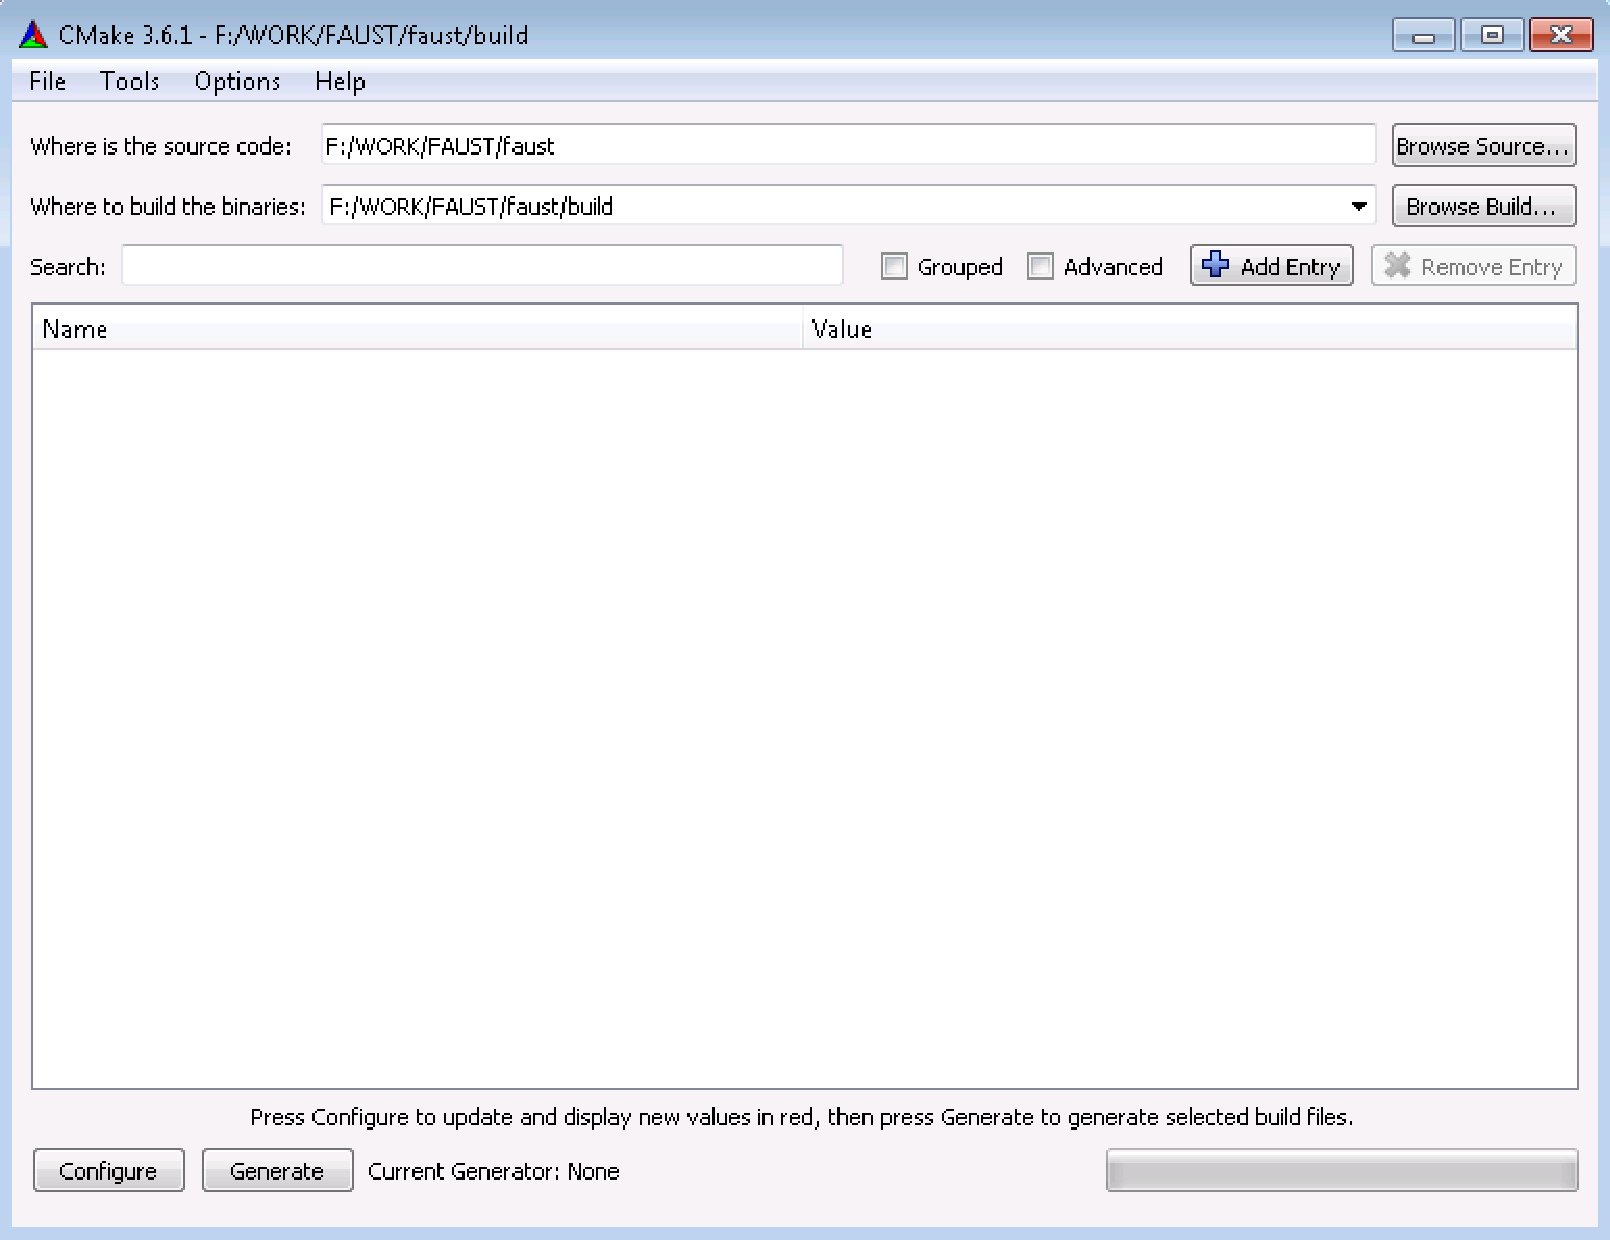
\includegraphics[scale=0.5]{images/cmakeGUI-1-eps-converted-to.pdf}
\caption{cmake GUI}
\label{fig:cmakeGUI-1}
\end{figure}

\item Set the "Where is the source code:" text box with the path of the directory where the source files are located (F:/WORK/FAUST/faust) and the "Where to build the binaries:" with the path of the directory where you want to build the library and executable files (F:/WORK/FAUST/faust/build). (see fig.  \ref{fig:cmakeGUI-1}).

When clicking for the first time on the [Configure] button, CMake will ask for the build tool you want to use. The build system type depends on the builder you want to use, in our case this is the Visual Studio X (X depending the version of Visual installed on the computer) chain tools. (see fig. \ref{fig:cmakeGUI-2}).


\begin{figure}[!h]
\centering
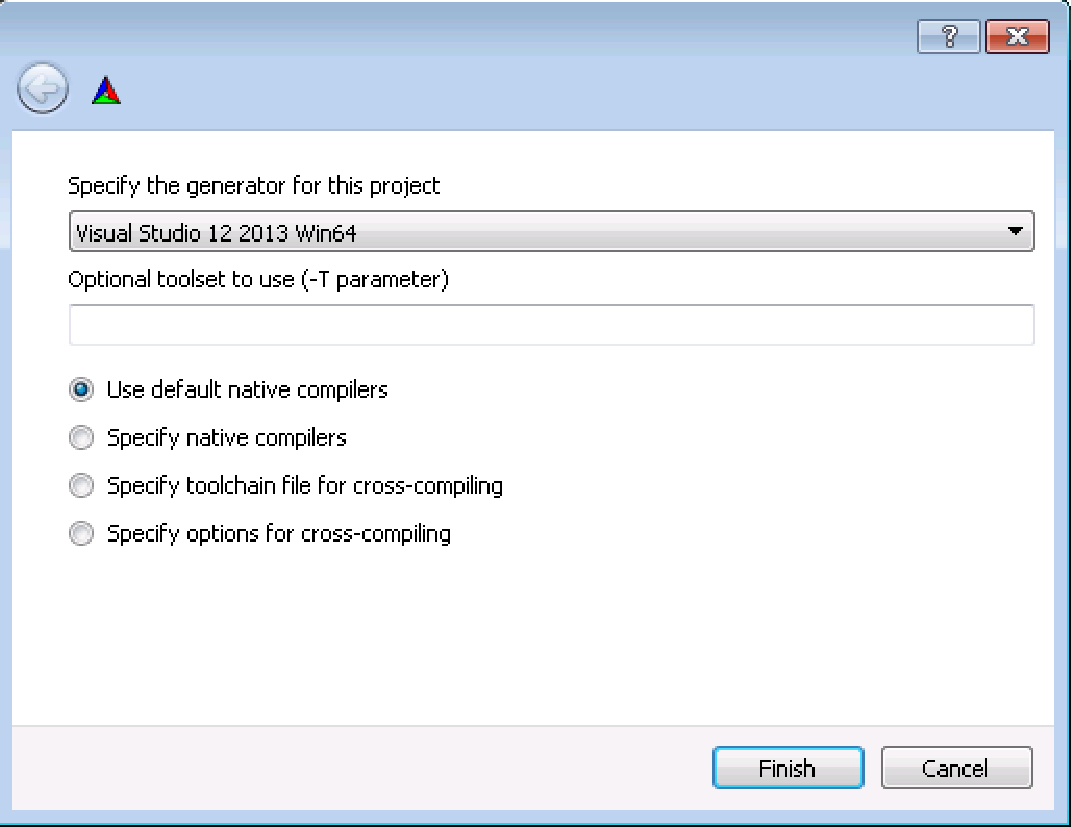
\includegraphics[scale=0.5]{images/cmakeGUI-2-eps-converted-to.pdf}
\caption{cmake GUI}
\label{fig:cmakeGUI-2}
\end{figure}

\item When pressing again the [Configure] button to configure the build system, CMake performs a list of tests to determine the system configuration and manage the build system. If the configuration is correct then no pop-up will appears during the tests and CMake finally shows the various options of the build underlaid in grey. In case of a configuration issue, a pop up window warns you about this issue indicating which test has failed, in this case the build option in the CMake application software will be underlaid in red. We will discuss in Section \ref{sec:WinCustomInstall} what to do in such a case, but let us for the moment assume that everything ran smoothly.
(see \ref{fig:cmakeGUI-4}).

\begin{figure}[!h] %%[!htbp]
\centering
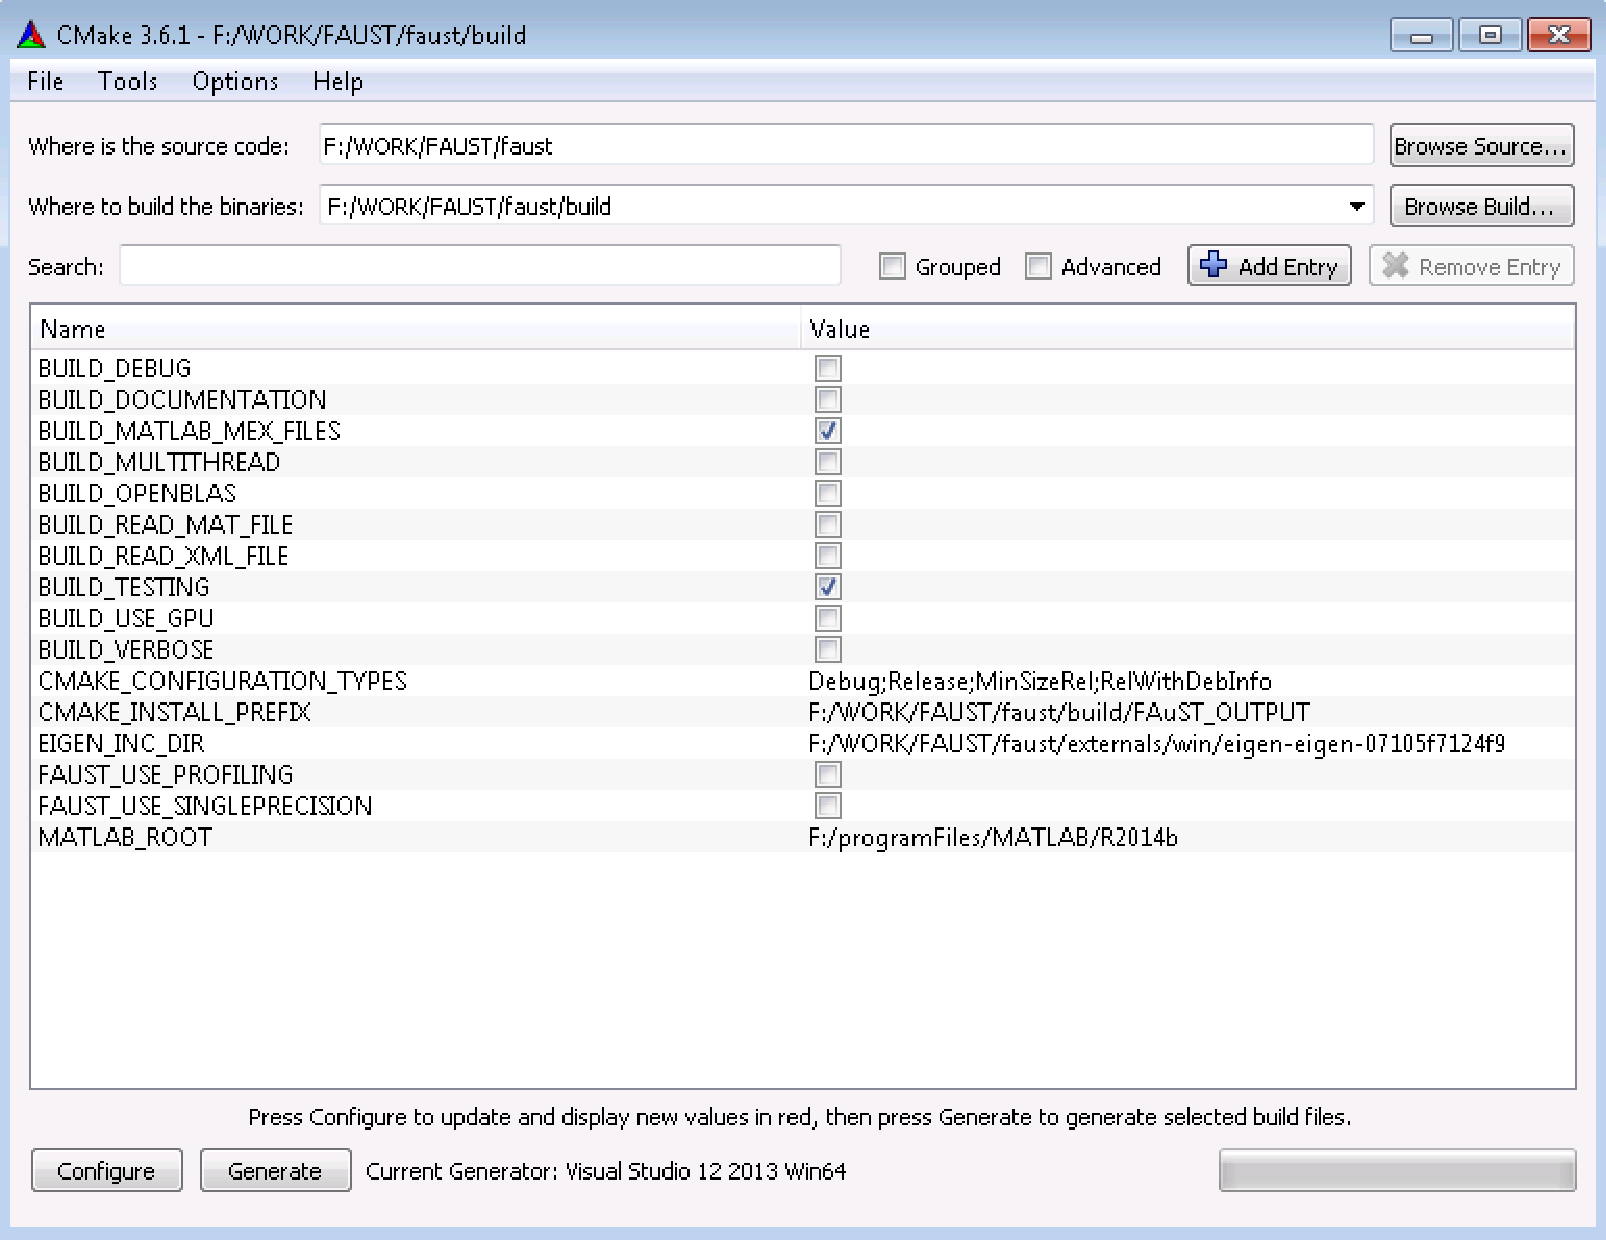
\includegraphics[scale=0.5]{images/cmakeGUI-4-eps-converted-to.pdf}
\caption{cmake GUI}
\label{fig:cmakeGUI-4}
\end{figure}

\item Once the build system configured then generated, you have to actually build FAUST, using Visual Studio.
\item Open file "faust.sln" with visual studio 
\item Click right on Target ALL\_BUILD and select generated 
\item Click right on Target INSTALL and select generated 
\item Click right on Target CTEST and select generated 
\end{enumerate}



\paragraph{}In the case of \textbf{Microsoft Visual Studio 2013 compiler using the command terminal} :

\begin{itemize}
\item Open a command terminal
\item Place you in your local FA$\mu$ST directory (NOTE: don't use any special character in your FAUST directory path, for example the character $\mu$)
\item Type the following commands : 

\begin{lstlisting}
mkdir build
cd build
cmake .. 
cmake --build . --config "Release" --target "install"
\end{lstlisting}

\end{itemize}

\section{Custom - Advanced Installation}\label{sec:WinCustomInstall}

progress... 



